\documentclass[DIV12,english,11pt,halfparskip]{scrartcl}
\usepackage[pdftex]{graphicx}
\usepackage[latin1]{inputenc}
\usepackage[headsepline]{scrpage2}
%\usepackage{amsmath}
%\usepackage{amssymb}
\usepackage{graphicx}
\usepackage{xcolor}
\usepackage{natbib}
%\usepackage{subfigure}
\usepackage[pdfpagemode=None,%
%linkbordercolor = 0 0 0,%
linkcolor = red,%
%anchorcolor = 0 0 0,%
citecolor = blue,%
%filecolor = 0 0 0,%
%5menucolor = 0 0 0,%
%pagecolor = 0 0 0,%
urlcolor = violet,%
colorlinks,%
plainpages=false, pdfpagelabels,%
%backref,%
pdftitle={JANE - Administration GUI},%
pdfsubject={},%
pdfauthor={Katrin Tomanek},%
pdfkeywords={Jena Annotation Environment, JANE},%
pdfcreator={JULIE Lab, University of Jena},%
pdfproducer={pdfeTeX},%
]{hyperref}
\pagestyle{scrheadings}
\automark{section}




\title{JANE -- Administration GUI}

\author{\normalsize Katrin Tomanek\\
  \normalsize  Jena University Language \& Information Engineering (JULIE) Lab\\
  \normalsize F\"urstengraben 30 \\
  \normalsize D-07743 Jena, Germany\\
  {\normalsize \tt katrin.tomanek@uni-jena.de} } \date{}

\begin{document}
\maketitle
\newpage
\tableofcontents
\newpage


\section{Introduction}


This documentation is a user howto for the administration GUI of JANE.
Throughout the documentation it is assumed that JANE is properly
installed.  For installation instructions of JANE please refer to the
installation howto.

As with the rest of JANE, the administration GUI has only been tested
on a Linux environment. JANE is implemented in Java and could therefore
also be run on a Windows machine. However, in this case the
configuration settings (especially paths) will have to be changed
accordingly.\footnote{Please note that we won't be able to help you
  running JANE on Windows...}


\subsection{Jena Annotation Environment}

The \emph{administration GUI} is part of the \emph{Jena Annotation
  Environment} (JANE) which is a platform that supports the complete
annotation life-cycle and allows for `focused' annotation based on
active learning -- an intelligent selective sampling strategy that
helps reduce the amount of data to be annotated substantially at
almost no loss in annotation effectiveness.

JANE consists of several components, \textit{viz.} one central
component, the annotation repository, where all annotation and project
data is stored centrally, two user interfaces, namely one for the
annotators and one for the administrator, and the active learning
component (currently for named entity annotations only) which
interactively generates documents to speed up the annotation
process. For a more detailed overview to JANE and its features, please
refer to \cite{Tomanek2007law}.


\subsection{About this Document}

This document is structured as follows: in the second section login to
the administration GUI is discussed, section three addresses user
management in JANE. Section four is on the management of annotation
projects, including their compilation, monitoring, and deployment.
Section five gives an overview to the log files written by JANE.
Finally, Appendix \ref{appendix:terminology} comments on underlying
ideas and concepts of JANE. You should check this section if you are
new to JANE.  Appendix \ref{appendix:preparation} discusses how to
prepare the data for annotation projects. If you want to create your
own annotation projects, you should carefully read this section.


\section{Running the Administration GUI}
In the directory \url{bin} of your \textsc{JANE} installation you will
find several command-line scripts. Run the administration GUI by
executing the following script: \url{runAnnoMaster.sh}.

\subsection{Login}
The administration GUI now starts with a user login (figure
\ref{fig:login}). All users which are currently added in the
annotation repository are shown here. After successfull login, the
main frame of the administration GUI will open.

\subsection{Logout}
Please note, that an administrator can only login once. This is a
necessary feature to avoid data inconsistency. Thus, you should close
the GUI properly and not just ``kill'' the GUI window. Only then the
user is logged out correctly. In case you did not logout properly (or
the GUI crashed for some reason), there is another command-line script
which can be used to logout a user: \url{logoutUser.sh}. Please, use
this script carefully always making sure that the user really should
be logged out!


\begin{figure}[h]
  \centering
  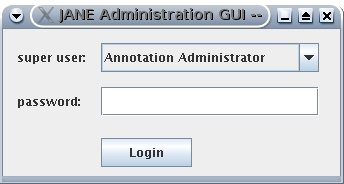
\includegraphics[scale=0.7]{figs/AnnoMasterLogin.jpg}
  \caption{Annotation GUI login}
  \label{fig:login}
\end{figure}



\section{User Management}

To create accounts for annotators, go to
\emph{Create$\rightarrow$User} at the menu bar. A new window pops up
(figure \ref{fig:createuser}) where you have to enter the login name,
a password and the full name of the new annotator.

\begin{figure}[h]
  \centering
  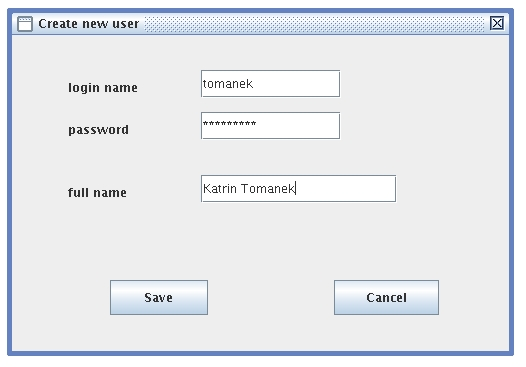
\includegraphics[scale=0.5]{figs/CreateUser.jpg}
  \caption{Creating an annotator account.}
  \label{fig:createuser}
\end{figure}

To see a list of all users of JANE (both annotators and the
administrator), go to \emph{Show$\rightarrow$User} at the menu bar.
You will get some information on each user, especially whether he is
currently logged in and his last login date (figure
\ref{fig:showusers}).

\begin{figure}[h]
  \centering
  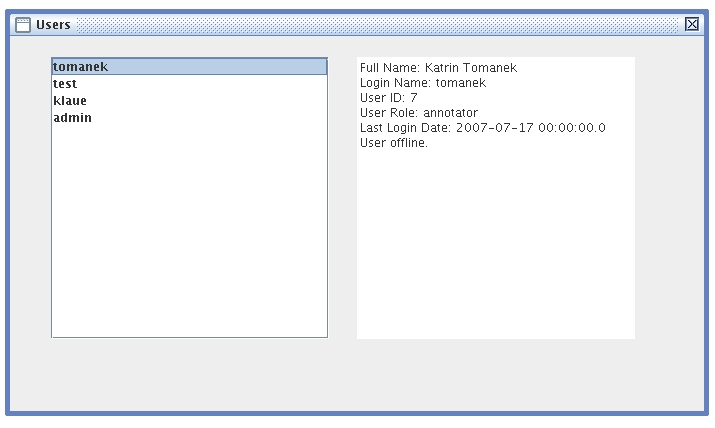
\includegraphics[scale=0.5]{figs/ShowUsersFrame.jpg}
  \caption{List of users.}
  \label{fig:showusers}
\end{figure}


\section{Annotation Project Management}

Project management comprises the creation and maintanance of
annotation projects, and deployment of annotated material.

\subsection{Creating a Project}

To create a new project, go to \emph{Creare$\rightarrow$Project} at
the menu bar. A new window will pop up where you have to specify all
project specific details and upload data. The new window is actually a
tabbed pane.  Each tab must be filled in before you can proceed to the
next one.  There are four tabs: \textit{general settings}, \textit{AL
  settings}, \textit{annotation schemata}, and \textit{documents}.
Projects are finally created by finishing the last tab. The previous
and next buttons on each tab provide a way to navigate between them.
It is also possible to go back and change previous entries.
Furthermore, creating a default project differs from AL project
creation. The tab \textit{AL settings} is not to be filled in for
default projects and is therefore skipped.

Note: Refer to appendix \ref{appendix:terminology} in case you need
more explanation of the single parameters that have to be specified or
files to be uploaded. Further, for information on how to get the data
you will need to upload here, please refer to appendix
\ref{appendix:preparation}.


\subsection{Creating a Default Project}
This subsection shows how to create a default project. First, you have
to specify general settings (figure
\ref{fig:createproject_generalsettings}). Select the annotator to
which the project should be assigned, specify a name for the new
projects (not more than 20 characters, overlong names will be cut),
select the priolist, choose the project type (default project here),
and finally add a short, explanatory description (do not use special
characters).

\begin{figure}[h]
  \centering
  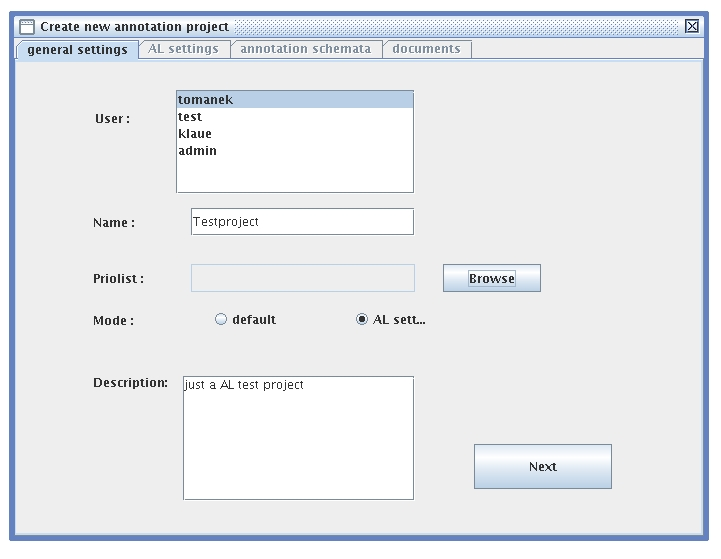
\includegraphics[scale=0.5]{figs/CreateProjectGeneralSettings.jpg}
  \caption{Create new annotation project -- general settings.}
  \label{fig:createproject_generalsettings}
\end{figure}

Second, you have to specify and upload the annotation schemata (figure
\ref{fig:createproject_annoschemata}.  You have to add at least one schema
file to the project. 

Pressing the add button pops up a dialog (see figure
\ref{fig:createproject_annoschema}) where you have to specify the
schema: define the annotation schema file, the respective
customization file, the level name (use the same name as used in the
files for the name space), and specify whether this annotation schema
is your main level (only one schema can be the main level and you have
to specify exactly one schema as your main level).


\begin{figure}[h]
  \centering
  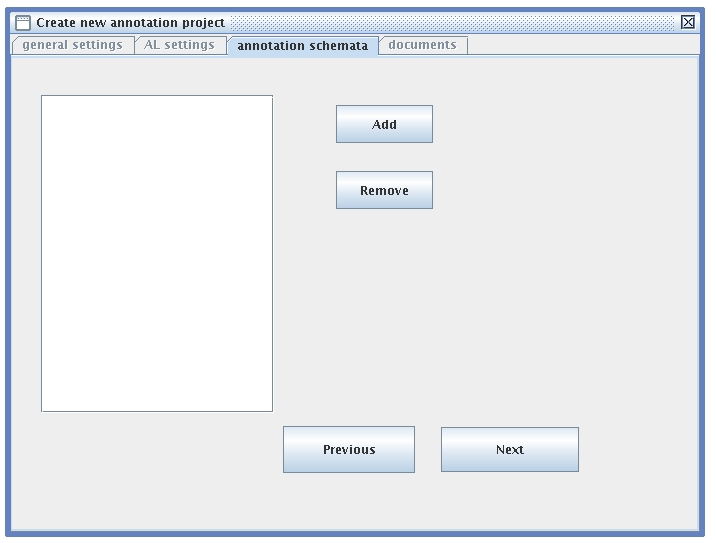
\includegraphics[scale=0.5]{figs/CreateProjectAnnotationSchemata.jpg}
  \caption{Create new annotation project -- add annotation schemata.}
  \label{fig:createproject_annoschemata}
\end{figure}

\begin{figure}[h]
  \centering
  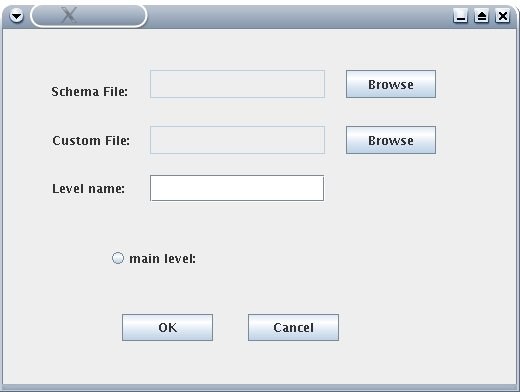
\includegraphics[scale=0.5]{figs/AddSchemataDialog.jpg}
  \caption{Create new annotation project -- adding a single annotation
    schema.}
  \label{fig:createproject_annoschema}
\end{figure}

Third, you need to upload the documents (basedata files) which should
be annotated. The last tab lets you add single and multiple documents,
and remove single documents (figure \ref{fig:createproject_documents}).

\begin{figure}[h]
  \centering
  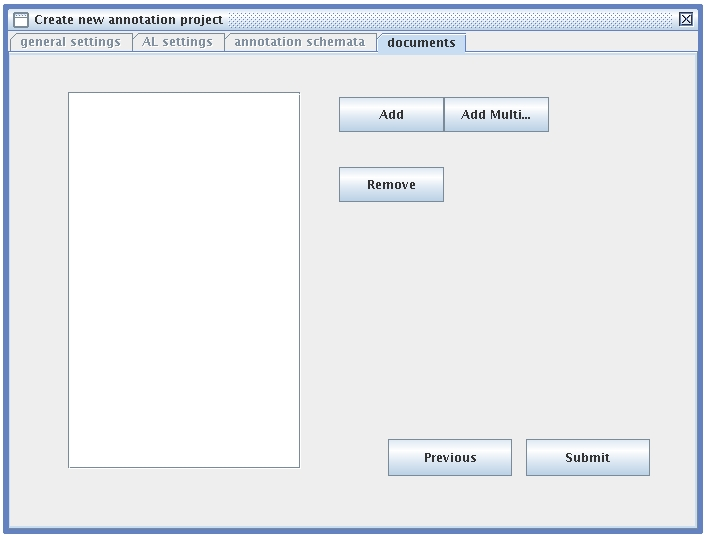
\includegraphics[scale=0.5]{figs/CreateProjectDocuments.jpg}
  \caption{Create new annotation project -- adding documents}
  \label{fig:createproject_documents}
\end{figure}

Adding a single document, you will have to specify the following
settings (figure \ref{fig:createproject_addsingledoc}):

\begin{itemize}
\item basedata file -- the respective MMAX2 file.
\item style file -- a style file, might be the default style file for
  default projects (for AL projects you must upload the special style
  file containing the context).
\item seed set -- only needed for AL projects (this is the
  alsessions.txt file, see appendix \ref{appendix:preparation}).
\item URI -- name of this document 
\item levels -- add a markable file for each annotation schema (level)
\end{itemize}

\begin{figure}[h]
  \centering
  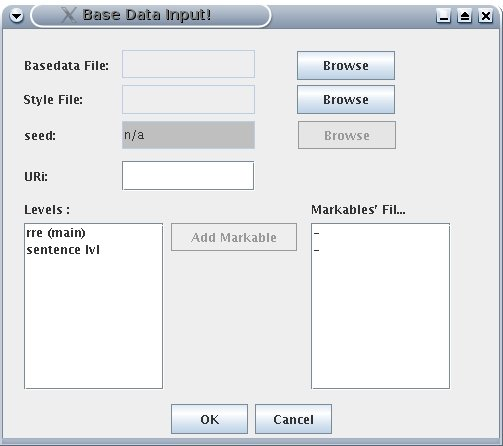
\includegraphics[scale=0.5]{figs/AddBaseDataDialog.jpg}
  \caption{Create new annotation project -- adding a single document.}
  \label{fig:createproject_addsingledoc}
\end{figure}


If you have a large number of documents to be added to your project
(this is only possible for default projects), just click on \emph{Add
  Multi}. Now you will have to specify some directories from which the
documents will be uploaded and their specifications will be derived
(figure \ref{fig:createproject_addmultidoc}):
\begin{itemize}
\item style file -- a style file (valid for all your documents to be uploaded)
\item basedatas -- a directory with a list of basedata files
\item markables -- a directory with markables which has to have the
  following structure: there have to be direct subdirectories with the
  names of the annotation schemata defined for this project. Each of
  these subdirectories has to contain the respective markables for
  this level for each basedata file (with the same name as the
  basedata file). Refer to the example data which is contained in
  directory \url{demo/default_project}.
\end{itemize}

If your specifications are correct, the bottom text area will show the
found basedata and markable files.


\begin{figure}[h]
  \centering
  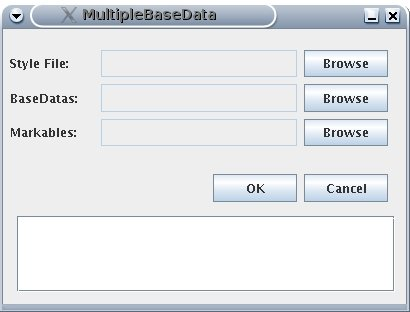
\includegraphics[scale=0.5]{figs/AddMultipleBaseData.jpg}
  \caption{Create new annotation project -- adding multiple
    documents.}
  \label{fig:createproject_addmultidoc}
\end{figure}


Since this is the last tab, project creation is finished here. If
everything is filled in correctly the submit button appears and if
invoked, inserts the new project into the annotation repository. If
you cancel, nothing is written to the database.


\subsection{Creating an AL Project}
In this subsection, we will show how to create an AL project. However,
only those tabs different from the ones when creating a default project
are shown. Make sure that when you create an AL project, you select AL
mode in the first tab.

Your second tab here will be on AL specific settings (figure
\ref{fig:createproject_ALsettings}). The following parameters have to
be specified (good default values are given in brackets):

\begin{itemize}
\item batch size -- number of sentences to be selected in each AL
  round (30)
\item fraction -- percentage sentences from the document pool to be
  considered in each AL run (0.01, but highly dependent on you pool
  size, select this value so that about 20,000 - 40,000 sentences are
  considered)
\item corpus BIN -- the binary corpus, choose the file
\item corpus TOK -- directory with original texts in tokenized form
\item corpus POS -- directory with original texts in POS-tagged form
\item labels -- file with labels (including outside label ``O'')
\item committee -- composition of committee for AL selection (keep
  default value ``ME,ME,ME'' unless you really know what you are doing)
\item training proportion -- percentage of data used to train each
  committee member (use default value ``0.65'' unless you really know
  what you are doing)
\end{itemize}


\begin{figure}[h]
  \centering
  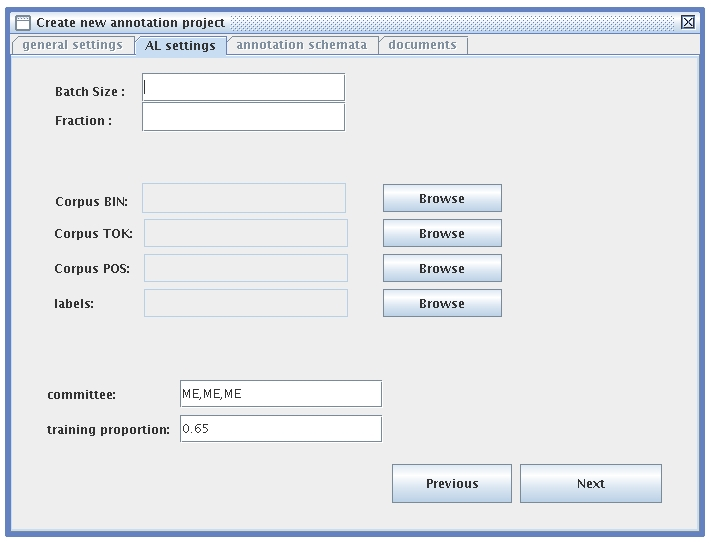
\includegraphics[scale=0.5]{figs/CreateProjectALSettings.jpg}
  \caption{Create new annotation project -- AL settings}
  \label{fig:createproject_ALsettings}
\end{figure}

The other tabs will be the same except that you can add only one
document, i.e. the seed set for AL.


\subsection{Showing Projects}

Go to \emph{Show$\rightarrow$Projects} at the menu bar to show all
projects in your annotation repository. A left click on a project
shows project details, a right click opens the \emph{project menu}
which lets you edit and monitor projects, and deploy the annotations.


\subsubsection{Modifying Projects}

To modify the settings of a project choose \emph{Edit} from the
project menu (figure \ref{fig:showprojects_edit}). All single
operations are self-explanatory. However, be carefull when deleting
and resetting projects as you won't be able to undo this operation.

\begin{figure}[h]
  \centering
  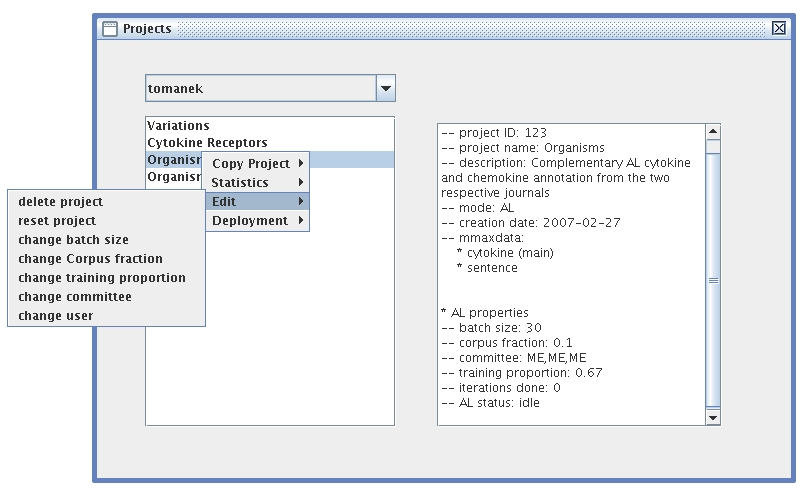
\includegraphics[scale=0.5]{figs/ShowProjects_Edit.jpg}
  \caption{Modifying annotation project specifications.}
  \label{fig:showprojects_edit}
\end{figure}

\subsubsection{Monitoring and Statistics}

Choosing \emph{Statistics} from the project menu you will find the
following options (figure \ref{fig:showprojects_stats}):

\begin{itemize}
\item Annotation times -- JANE estimates the annotation time by the
  time MMAX2 is opened for a document. Only documents set to status
  ``done'' are considered when calculating the average.

\item AL selection time -- an overview of the time needed to perform
  AL selection, split into several steps (training, making the
  training data, prediction, making the prediction data). Overall
  selecion time also subsumes other steps (e.g. reading the binary
  corpus).

\item Cumulated entities -- plots the overall number of entities
  annotated and the number of distinct entities annotated (only
  documents set to status ``done'' are considered). This is a valuable
  hint of annotation project progress, especially for AL projects.

\item Disagreement -- two different disagreement statistics are shown
  here: selected sentence disagreement (the average disagreement of
  the committee on the selected sentences) and overall disagreement
  (the average disagreement of the committee of all sentences during
  one AL round). Disagreement is an important predictor when AL-based
  annotation can be stopped. See \cite{Tomanek2007emnlp} for more
  details.
\end{itemize}

\begin{figure}[h]
  \centering
  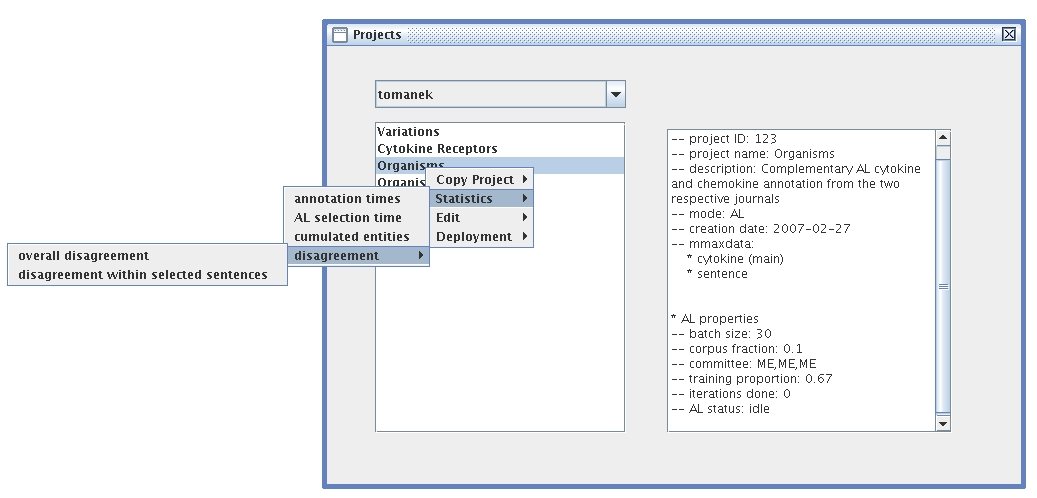
\includegraphics[scale=0.5]{figs/ShowProjects_Statistics.jpg}
  \caption{Showing statistics on annotation projects.}
  \label{fig:showprojects_stats}
\end{figure}


\subsubsection{Deployment}

Choosing \emph{Deployment} from the project menu you will find the
following options (figure \ref{fig:showprojects_deploy}):

\begin{itemize}
\item Export to t2 format -- only for AL projects. The t2 format is
  similar to the well-known IOB format. Each line contains a token and
  its respective label. Sentences are separated with empty lines. In
  contrast to the IOB format, files in the t2 format, each sentence
  has a header in the following form: ``SENTENCE 11319234 9 33'',
  where the first number is the URI (text id), the second number the
  sentence number, and the third number specifies the length of the
  sentence in terms of tokens.

  For each AL project the current annotations are kept in t2 format in
  the annotation repository. You can download the annotations into a
  file using this option.

\item Convert and export to t2 format -- For non-AL projects, you can
  create the annotations in the t2 format by choosing this option.
  Only documents where the status was set to ``done'' are considered
  here.

\item Convert and export to IOB format -- converts the annotated
  documents (status ``done'') of a project into the IOB format.
  Actually, at the moment no begin labels are assigned (might come in
  a later version). So, just the outside label ``O'' and the entity
  labels as defined in the priolist are used.

\item Export main markables -- saves all markables of the main
  annotation scheme (respective documents set to ``done'') to the
  specified directory.
\end{itemize}

\begin{figure}[h]
  \centering
  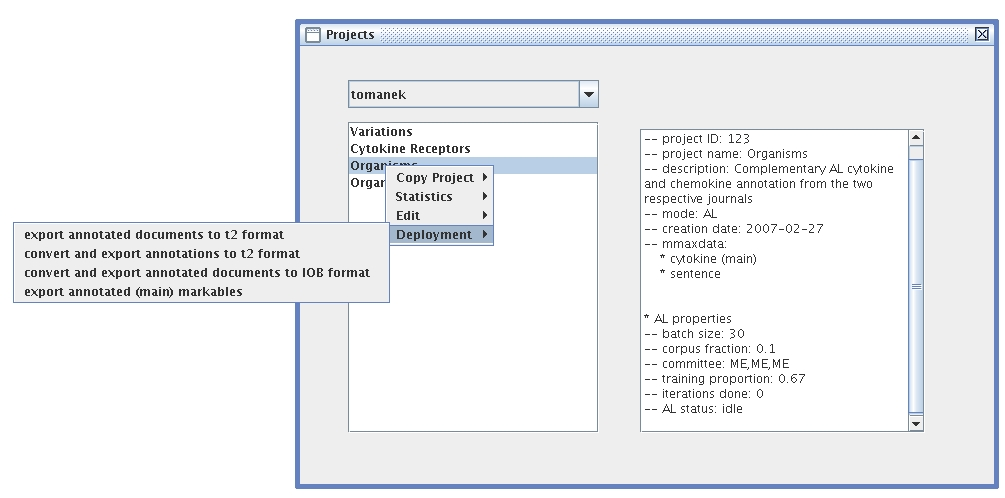
\includegraphics[scale=0.5]{figs/ShowProjects_Deploy.jpg}
  \caption{Deploying annotated data.}
  \label{fig:showprojects_deploy}
\end{figure}

\section{Viewing Logfiles}

In JANE, many operations of the administration GUI, user login and
logout, and single steps of the AL selection process, as well as
errors and warnings are stored in a special log table in the
annotation repository. Go to \emph{Show$\rightarrow$Logs} at the menu
bar to see JANE's log entries (figure \ref{fig:showlogs}).


\begin{figure}[h]
  \centering
  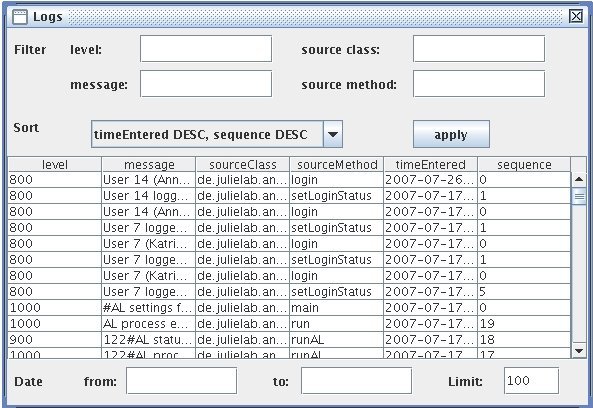
\includegraphics[scale=0.5]{figs/ShowLogs.jpg}
  \caption{JANE's log files.}
  \label{fig:showlogs}
\end{figure}

There are the following log levels: 800 means information, 900 means
warning, and 1000 means error. You might every now and then check the
log files for errors or warnings.

You can set filter rules to show only some log entries. In the
\emph{message}, \emph{source class}, and the \emph{source method}
filter, you can use ``\%'' as a wildcard for a sequence of arbitrary
characters.

Further, you can restrict the number of log entries returned. Per
default, only 100 entries will be shown.


%-----------------------------
 \newpage
\begin{appendix}
\appendix
%-----------------------------

\setcounter{figure}{0}
\section{Fundamentals and Principles}
\label{appendix:terminology}

In this section you will find a more detailed explanation of concepts
and principles of JANE.

\subsection{General Terminology}

In JANE, an \textbf{annotation project} consists of a
\textbf{collection of documents} to be annotated, an associated
\textbf{annotation schema} -- a specification of what has to be
annotated in which way, according to the accompanying annotation
guidelines -- a set of configuration parameters, and an
\textbf{annotator} (or \textbf{user}) assigned to it. 

We distinguish two kinds of annotation projects: A \textbf{default
  project}, on the one hand, contains a predefined and fixed
collection of naturally occurring documents which the annotator
handles independently. In an \textbf{active learning
  (AL) project}, on the other hand, the annotator has access to
exactly one (AL-computed pseudo) document at a time. After such a
document has completely been annotated, a new one is dynamically
constructed which contains those sentences for annotation which are
the most informative ones for training a classifier.  Besides
annotators who actually do the annotation, there are
\textbf{administrators} who are in charge of (annotation) project
management (see administration GUI howto).


\subsection{MMAX2 as External Annotation Editor}
In JANE, annotation itself is based on the external annotation editor
MMAX2\footnote{\url{http://mmax2.sourceforge.net}}. Profound knowledge
of MMAX2, especially how to create MMAX2 projects,\index{} is assumed.
Please refer to the respective documentation of MMAX2.  You should
especially be familiar with the following MMAX2 files, as they are
used by JANE\footnote{JANE's database schema mirrors MMAX2 project
  data structure, i.e., the files MMAX2 needs for a project.}:

\begin{itemize}
\item basedata
\item markable (often referred to as ``level'' in JANE)
\item annotation scheme (referred to as ``schema'' in JANE)
\item customization (referred to as ``customization file'' in JANE)
\item style file
\end{itemize}


\subsubsection{Annotation Schemes in JANE's Annotation Projects}

Typically, in our annotation projects we have several annotation
schemes (and accordingly we have several markables, one for each
annotation scheme).

We found it beneficial to have one sentence per line in the MMAX2
editor. To accomplish this, we always add a so-called
\textbf{sentence-level markable} containing the offsets the sentences
(the respective annotation schema and customization files can be
empty).

AL projects \emph{must} have this! For default projects, it is
optional, although, our command-line scripts for preparing default
projects (see appendix \ref{appendix:preparation}) will always create
the sentence level.

When creating a new project with the administration GUI, exactly one
annotation scheme (level) has to be set as the \emph{main level}.
This should never be your sentence level annotation scheme but the
entity-level scheme, i.e., the one on which you are actually doing you
annotations.

In the directory \url{demo/default_project/Markables/sentence/}
(available in the SVN repository of JANE) you will find examples for
such an sentence-level markable.



\subsubsection{Context in AL Projects}
In AL projects the annotator is shown the original context in which a
selected sentence occurs. This context is put into the MMAX2 style
file -- it is shown in the MMAX2 editor in italics and cannot be
annotated.

Before creating a new AL project with the administration GUI, you will
have to prepare your project data accordingly, i.e. amongst other
things, you will have to set up an initial style file containing the
context of your seed set. Appendix \ref{appendix:preparation} explains
how this can be done with the command-line scripts.


\subsection{Annotation Projects}

In context of annotation projects, several terms need further
explanation.

\subsubsection{Default and AL Projects}

\begin{description}
\item[priolist] each annotation project has a list where the
  entity-labels are given a priority. This priority specification is
  used when the MMAX2 data is converted into other formats. This is
  the case during AL-selection (see below) and when exporting the
  annotations. When there are overlapping annotation, i.e. if one
  token has more than one annotations, the longest annotation is used.
  If, however, several annotations of same length are specified, the
  order in the priolist decides which label to choose.

  Further, only those labels contained in the priolist will be
  considered during data conversion. Thus, if you e.g.\ want to
  restrict the entities/labels to be considered during AL-selection,
  just use an incomplete priolist.

  Not only AL projects, but also default projects have such a
  priolist. There, the priolist is only used during annotation
  export/deployment.
\end{description}




\subsubsection{AL Projects}

In this subsection, the most important concepts related to AL projects
are described. For a general understanding of how AL selection works
please refer to \cite{tomanek.thesis10}.

\begin{description}
\item[main level] the annotations of this annotation scheme (level)
  are considered during AL selection. You always need to have one main
  level (which must not be the sentences level).
\item[labels] specify the labels (same as in the priolist) to be
  considered during AL. Add an extra label, the ``outside'' label
  (which has to be ``O''). Although this is somewhat
  redundant\footnote{We will probably remove the ``labels'' in a later
    version of JANE.}, make sure you specify the labels carefully.
\item[batch size] the batch size specifies the number of sentences
  that are selected in each AL. In theory, the smaller the batch size,
  the better AL works. However, experiments have shown, that the batch
  size doesn't really affect the AL performance too much. 

  Thus, other considerations might lead you when specifying the size.
  We found that it is more motivating for our annotators to have
  moderate batch sizes (30-50 sentences).

\item[fraction] AL selection has in background a large pool\footnote{A
    document pool with several hundreds of thousands of sentences is
    quite a realistic settings.} of unlabeled documents from which it
  selections sentences for annotation. To speed up AL selection, we
  only consider a random subsample during each AL round. The
  \emph{fraction} defines which percentage of the sentences of the
  document pool to consider (see below: binary corpus).

  We typically specify this value so that about 20,0000 to 40,000
  sentences are considered.

\item[binary corpus] the document pool is stored in a specific binary
  format which allows to select a random subsample from it very
  efficiently (see above: fraction). To accomplish this, the sentences
  of the binary corpus are transformed to have the same length.
  Appendix \ref{appendix:preparation} explains how to construct such a
  binary corpus from your data.

\item[committee] our AL selection is based on a committee of three
  classifiers. You can specifiy the learning algorithm of each of
  these classifiers. Allowed values are: NB (Naive Bayes), ME (Maximum
  Entropy), CRF (Conditional Random Fields), and MEMM (Maximum Entropy
  Markov Models). 

  We propose to use a homogeneous committee of ME classifiers as it is
  a good compromise between speed and AL performance. Of course, you
  can also employ a heterogeneous committee (e.g. with a ME, a CRF,
  and a MEMM classifiers). However, we found this not to improve the
  performance significantly.

\item[training proportion] In every AL round, each classifier of your
  committee will be retrained on the material you have annotated so
  far in the current project. The training proportion specifies the
  percentage of annotated data to be used to train each classifier.

  In case of a homogeneous committee, i.e. one that consists of
  classifiers of the same learning algorithm, you \emph{must} choose
  training proportion clearly smaller than $1$ otherwise AL selection
  will equal random selection.

  We propose to use a training proportion of $\approx 0.67$ for
  homogeneous committees. In a heterogeneous committee, the training
  proportion should be set to $1$.


\item[seed set] a seed set specifies the sentences that should be
  considered in the initial AL round. When preparing the data for an
  AL project (see appendix \ref{appendix:preparation} you have to
  specify the seed set. A proper seed set is important for good AL
  performance \cite{Tomanek2007law}.

\end{description}



%------------------------------------
\section{Preparing Project Data}
\label{appendix:preparation}
%-----------------------------------


This section explains how to prepare the data which needed to create
new annotation projects. The administrator is supported with some
scripts which can be found in the subdirectory \url{bin}.

\subsection{Preparing Default Projects}


This is a short description about the preparation steps necessary to
create a default project with multiple basedata.Lets assume, that you
have a collection of (tokenized and sentence splitted, one sentence
per line) and you want to create a default annotation project with one
document for each of these files. Thus, you need to create one MMAX2
basedata file, a sentence-level schema, and a entity-level schema for
each of your input files. To speed up this process, there is a script
(see below) which does the work for you.

This is a step-by-step description how to prepare the data for such a
default project. Once you have created the data, you can create a new
projects from the administration GUI (see above). 

First, define your entity-level annotation scheme and the respective
customization file accordings to the MMAX2 guidelines. See figures
\ref{fig:muc_schema} and \ref{fig:muc_cust} for the files for the MUC
example (person, location, and organization annotation).

\begin{figure}[h]
\begin{verbatim}
<?xml version="1.0" encoding="UTF-8"?>
<annotationscheme>
  <attribute id="muc" name="muc" text="" type="nominal_button">
    <value id="organization" name="organization"/>
        <value id="person" name="person"/>
        <value id="location" name="location"/>
   </attribute>
</annotationscheme>
\end{verbatim}
\label{fig:muc_schema}
\caption{entity-level annotation scheme for MUC example}
\end{figure}

\begin{figure}[h]
\begin{verbatim}
<?xml version="1.0" encoding="UTF-8"?>
<customization>
  <rule pattern="muc={person}" style="background=green"/>
  <rule pattern="muc={organization}" style="background=blue"/>
  <rule pattern="muc={location}" style="background=red"/>
</customization>
\end{verbatim}
\label{fig:muc_cust}
\caption{entity-level customization for MUC example}
\end{figure}

Second, create the MMAX2 style file (you might use the MMAX2 style-file
template therefore, but don't forget set the namespace for your
annotation levels correctly).

Now use the script \url{manualTok2Mmax.sh} to create the missing
files. Calling the script without any parameters will tell you the
exact usage.

In the directory \url{demo/default_project/} you will find examples of
the files discussed in this subsection and other files necessary to
create the default project (priolist.txt, labels.txt, styles.xsl).


\subsection{Preparing AL Projects}

This is a short description on the single steps necessary to prepare
the data needed by an AL project. Once all data is created, use the
administration GUI to create a new project.

\subsubsection{Creating the Document Pool}
First, you need to create the document pool from which AL can select
single sentences for manual annotation.

Therefore, create a directory with files. Each file must have the
following form:
\begin{itemize}
\item one sentence per line
\item POS tags after a token (delimiter: ``\_''). A sentence might
  have the following form:
\begin{verbatim}
  Maruti_NNP holds_VBZ 70_CD percent_NN of_IN the_DT Indian_JJ car_NN
  market_NN ._.
\end{verbatim}
\end{itemize}

When a sentence is selected, the whole file in which it occurs is
shown to the annotator as context. As long as your files only contain
abstracts this is OK. However, when you e.g.\ work on full texts, you
should split them into single paragraphs (or sections, etc.) and store
each of them in a separate file. Make sure the file names only contain
numbers and no extension (and no other special characters).

\subsubsection{Creating a Binary Corpus}

Now, you need to convert this collection of files into a something we
call a \emph{binary corpus} (bincorpus): a binary version of your
files where each sentence has the same size (shorter sentences are
padded). We need this during AL selection where we pick a random
subsample of your corpus. The binary format of your corpus is
accessible very fast and thus essential to guarantee fast AL
selection.

Use the following script to create the binary corpus:
\url{createBinCorpus.sh}. Running the script with no parameters will
tell you which parameters to use.

Run the script once in inspection mode (use flag ``-i''). Note:
specify a large sentence size here; 4000 has been shown as a good
value (if it isn't enough use a larger number) to get the optimal
length (i.e., shortest possible length with respect to the longest
sentence in the corpus).

Now, use the number that was returned in investigation mode and add
$1$ (you might add some more bytes till you get a nicer number, maybe
some $2^n$) in a second run of the script (without flag ``-i'').

\textbf{Important note:} a binary corpus will easily occupy 3 GB of
disk space! Thus, make sure you have enough disk space.


\subsubsection{Creating the MMAX2 data}

As with the default projects, we now need to create the data for the
project.

First, you need to define which sentences should be used in the
initial AL round. Refer to \cite{Tomanek2007law} for a discussion why
a proper \emph{seed set} is important. Once you have decided on the
sentences to be used, create a file where you list the sentences to be
used in the following form:

\begin{itemize}
\item <file name> <sentence number>
\item file name as in the document pool (of POS tagged files)
\item sentence number starts from 0
\end{itemize}

Such a file might look like this:
\begin{verbatim}
387812 1
398888 7
907771 3
...
\end{verbatim}

As with the default project, define your entity-level annotation
scheme and the customization file. Use the script
\url{createALFiles.sh} to create the following files (call the script
without arguments to see the list of arguments and follow these
instructions):
\begin{itemize}
\item style file
\item basedata file
\item sentence-level markable
\item alsession.txt
\end{itemize}

Just pipe the output printed to STDOUT into a file.

Now, you create a new AL project with the help of the annotation GUI.


\end{appendix}

\bibliographystyle{unsrt}
%\bibliographystyle{alpha}
\bibliography{literature}


\end{document}
